\documentclass[border=0.8ex,svgnames,tikz]{standalone}
\usepackage{amsmath,mathtools}
\usepackage{fontspec}
\setmainfont{Source Serif 4}
\setsansfont{Source Sans 3}
\setmonofont{Source Code Pro}
\begin{document}
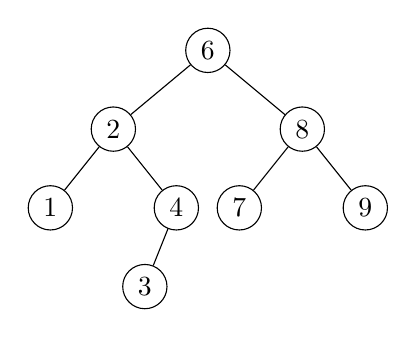
\begin{tikzpicture}[
  level distance=10mm,
  every node/.style={draw,circle,inner sep=1pt,minimum size=1.6em},
  level 1/.style={sibling distance=24mm},
  level 2/.style={sibling distance=16mm},
  level 3/.style={sibling distance=8mm},
  ]
  \node{6}
  child{
    node{2}
    child{ node{1} }
    child{ node{4} child{ node{3} } child[missing] }
  }
  child{ node{8} child{ node{7} } child{ node{9} } };
\end{tikzpicture}
\end{document}
